\documentclass[twocolumn,10pt]{article}

\usepackage[a4paper,hmargin=1.5cm,vmargin=2.5cm,]{geometry}
\setlength{\columnsep}{0.7cm}
\usepackage{amsmath}
\usepackage{graphicx}
\usepackage[utf8]{inputenc}
\usepackage{hyperref}
\urlstyle{same} % no tt font for URLs

\usepackage{natbib}
\bibliographystyle{genome_research}
%\setcitestyle{aysep={}} 

\usepackage[dvipsnames]{xcolor}
\hypersetup{
    colorlinks,
    linkcolor={blue!50!black},
    citecolor={blue!50!black},
    urlcolor={blue!50!black}
}
\renewcommand{\dbltopfraction}{0.7}
\renewcommand{\textfraction}{0.2}

\begin{document}

\setcounter{secnumdepth}{0}

\twocolumn[{%
\centering
\textbf{\Large Analysing single-cell bisulfite sequencing data with scbs}
\vspace{1.5ex}

Lukas P. M. Kremer, Leonie Küchenhoff, ..., Simon Anders\\
{\footnotesize University of Heidelberg, Germany}
\vspace{1.5ex}

March 2022
\vspace{6ex}
}]

\section{Comparison}

To demonstrate an improvement of results, we compare previously published analyses described above with our analysis method.
First, we use a dataset by \citealp{Argelaguet_2019}. In their work, they generated a single cell methylome dataset of mouse embryo cells across different stages of development (E4.5 – E7.5). They calculated the correlation between RNA expression intensity and corresponding DNA methylation at the promoter region to elucidate the implications of the epigenome on RNA expression during development. As promoters, they used DNA regions of $\pm$ 2kb around transcriptions start sites (TSS). 


--The following paragraph potentially needs to be changed when new plots are made--


In our analysis, we compare correlations between RNA expression intensity and DNA methylation of these promotor regions to correlations between RNA expression intensity and DNA methylation of the closest variable methylation regions that we identified with scbs. In figure \ref{figure:correlation}, we show that correlation of RNA expression intensity to gene methylation around the TSS $\pm$ 2kb is less strong compared to the correlation at the closest variable region. This effect can be observed with mehtylation fractions (figure \ref{figure:correlation}A) or shrunken residuals (figure \ref{figure:correlation}B) as data inputs.

\begin{figure}[!htp]
	A\\
	\hspace{.2cm}\includegraphics[width=.7\columnwidth]{leonie_plots/corr_methylation_fraction_4kbwindow.pdf} \\
	B\\
	\hspace{.2cm}\includegraphics[width=.7\columnwidth]{leonie_plots/corr_shrunken_residual_4kbwindow.pdf} \\
	C\\
	\hspace{.39cm}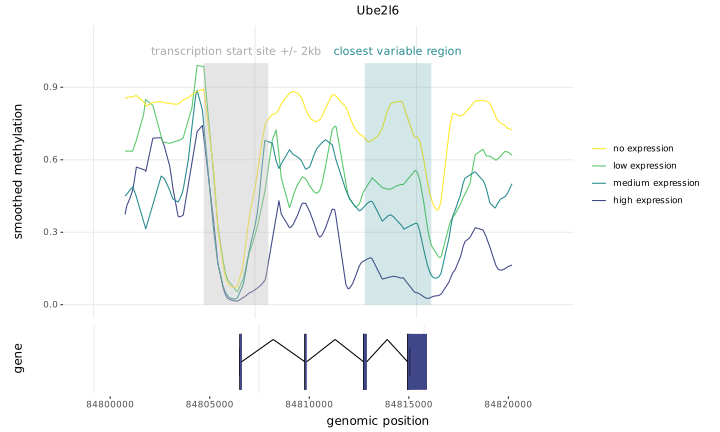
\includegraphics[width=\columnwidth]{leonie_plots/comparison_meth_RNA.pdf}

	\caption{\small \textbf{Correlation of DNA methylation and RNA expression intensity}. All plots are based on the data by \citealp{Argelaguet_2019}.
	\textbf{(A)} Correlation of each gene's RNA expression intensity to methylation fraction of TSS $\pm$ 2kb (y-axis) or to methylation fraction of closest variable gene.
	\textbf{(B)} Correlation of each gene's RNA expression intensity to shrunken residual of methylation of TSS $\pm$ 2kb (y-axis) or to shrunken residual of closest variable gene.
	\textbf{(C)} Mean gene methylation of Ube2l6 gene (ENSMUSG00000027078, marked in yellow in A \& B). Cells were into 4 groups based on their RNA expression (group 0: cells with no expression of gene, group 1-3: cells that express gene divided into three equally large groups with group 3 having the highest expression). Mean methylation level of each group was smoothed with a tricube kernel of bandwidth = 2000.}
	\label{figure:correlation}
\end{figure}

As an example to illustrate this effect more clearly, we picked a gene with significantly stronger correlation at the closest variable region than at the TSS. This gene is marked on figure \ref{figure:correlation}A and B with a yellow dot. We divided all cells into four groups of cells with no, low, medium and high expression of this exemplary gene Ube216 and plotted a smoothed methylation level per group. As shown in figure \ref{figure:correlation}C, the promoter region is sparsely methylated in all four RNA expression groups and is therefore a poor region to make conclusions about the relation of DNA methylation and RNA expression intensity. However, a region close to the TSS, identified as the closest highly variable methylation region with scbs, shows a much clearer negative correlation between RNA expression intensity and DNA methylation.  


To further demonstrate the benefit of detecting variable methylation regions, we used a second dataset, published by \citealp{Luo_2017}. In their work, \citealp{Luo_2017} generated methylomes from single cell neuronal nuclei in mice to identify genomic regulatory elements across neuron types. To compare how well cell types are separated by different analysis techniques, we processed the same dataset into 2-dimensional UMAPs several times. Subsequently, we compared the results by assigning a score to each output based on cell type separation in the final 15 principal components. We see an improvement of cell separation when comparing the analysis of variable methylation regions to 100 kb regions (\ref{figure:score}A and C). The difference of using shrunken residuals instead of methylation fractions to assess the methylation per region is not as significant. However, when emulating a sparse dataset with less cells by randomly reducing the dataset to 500 cells, it becomes clear that using shrunken residuals over methylation fractions also improves the outcome of our analysis (\ref{figure:score}B and D). 


\begin{figure}[!htp]
	A\\
	\hspace{.3cm}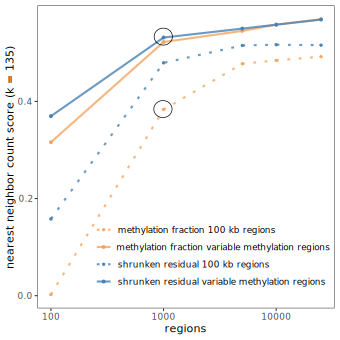
\includegraphics[width=.7\columnwidth]{leonie_plots/complete_135k_12cm_log.pdf} \\
	B\\
	\hspace{.3cm}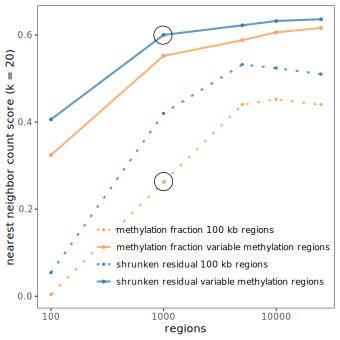
\includegraphics[width=.7\columnwidth]{leonie_plots/cell500_20k_12cm_log.pdf} \\
	C\\
	\hspace{.39cm}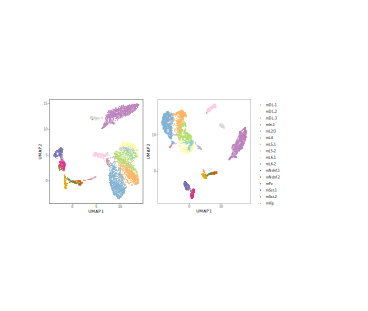
\includegraphics[width=\columnwidth]{leonie_plots/UMAP_fulldataset.pdf}
	D\\
	\hspace{.39cm}\includegraphics[width=\columnwidth]{leonie_plots/UMAP_reduceddataset.pdf}
	\caption{\small \textbf{Analysis comparison}. All plots are based on the data by \citealp{Luo_2017}. \textbf{(A)} Nearest neighbor count score for complete dataset using four different analysis techniques and a variable number of regions as input. Exemplary UMAPs for encircled scores are shown in (C). \textbf{(B)} Nearest neighbor count score for the same dataset reduced to 500 cells using four different analysis techniques and a variable number of regions as input. Exemplary UMAPs for encircled scores are shown in (D). \textbf{(C)} Two exemplary UMAPs using 1000 regions of the full dataset and methylation fraction of 100 kb windows (left) or shrunken residuals of variable methylation regions (right) \textbf{(D)} Two exemplary UMAPs using 1000 regions of the reduced dataset and methylation fraction of 100 kb windows (left) or shrunken residuals of variable methylation regions (right).}
	\label{figure:score}
\end{figure}


\section{Discussion and Conclusion}

...


\section{Methods}

\subsection{Data processing}
To analyze CpG methylation data by \citealp{Luo_2017}, the mouse genome was first separated into regions. Regions were either obtained by tiling the genome into non-overlapping 100 kb bins or by acquiring the most variable methylation regions with the scbs script as described above. For each region, the mean methylation fraction or methylation residual was calculated. Each region that contained less than four measured CpGs or that was measured in less than 10\% of cells was removed from the dataset. To select $n$ regions for further analysis, top $n$ regions were picked based on the cell number the region was measured in. 
For dimensionality reduction, missing values were imputed with an iterative PCA as described below. To visualize data, a UMAP was performed on the final 15 principal components.

\subsection{Scoring}
To assess data processing performance of several DNA methylation analysis techniques, we processed single cell DNA methylation data with several approaches and scored each result. Scores evaluate the ability of each method to separate cell types in a 15-dimensional space of the first 15 principal components based on their CpG methylation. Each score varies between 0 and 1, where higher scores reflect better data processing performance.
\subsubsection{Nearest Neighbor Count Score}
The nearest neighbor count score $nnc(k)$ is based on the $\Gamma -Score$ published by \citealp{Kireeva_2014}. Each cell $c_j^i$ belongs to a cell type $j$. For each cell, $k$ nearest neighbors $nn_j^k$ were computed based on their Euclidean Distance. Based on the cell type $j$ of the $k$ nearest neighbors of each cell, the nnc score $nnc(k)$ was computed with fomula (1), in which $d(c_j^i, k_j^i)=1$ if at least 90\% of neighbor classes match the class of cell $c_j^i$ and $d(c_j^i, k_j^i)=0$ if less than 90\% of classes match, while $n$ are the total number of cells.
\begin{equation}
	nnc(k) = \frac{1}{n}d(c_j^i, k_j^i)
\end{equation}



{\small \bibliography{scbs}}

\end{document}